\makeatletter
\def\maxwidth#1{\ifdim\Gin@nat@width>#1 #1\else\Gin@nat@width\fi}
\makeatother

\chapter{Introduction}

Automated testing has never been an outdated problem in mobile application developing process. There are over 2,500 manufacturer models and over 100 mobile operating system versions \cite{crittercism}. Daily developed mobile applications need to be tested in wide range of phone designs and platforms. These result in enormous amount of testing scenarios and require an effective industrial testing series. Current software-based testing method has shown some advantages but there are still some issues demanded to be dealt with.

The problem of present testing method is that only software aspect is considered. Tester can run test cases perfectly in software regardless hardware's failure like button or touch screen malfunction. Otherwise, each phone operating system requires different corresponding testing framework. These factors conspire to make the cross-platform mobile application testing very challenging. \nocite{weinman_thesis}

We propose a new approach that in its design, software and hardware testing are more integrated. Applying image processing technologies, our system can detect content of phone screen and produce actions on it. These actions are performed directly on target phone by delta robot. Robotics testing gives us a less invasive way of mobile testing that does not require special software on target phone. In addition, the testing series can be applied on any mobile phone operating systems without doubt.

\section{System overview}

The system overview and design are described below in Figure \ref{fig:system_overview}.

In this thesis, I developed and manufactured Delta robot and provides control API. The testing framework which is designed and constructed by my partner, \textit{Hieu} Nguyen Duc using my robot controller module to perform the work test.

\begin{figure}[H]
	\centering
	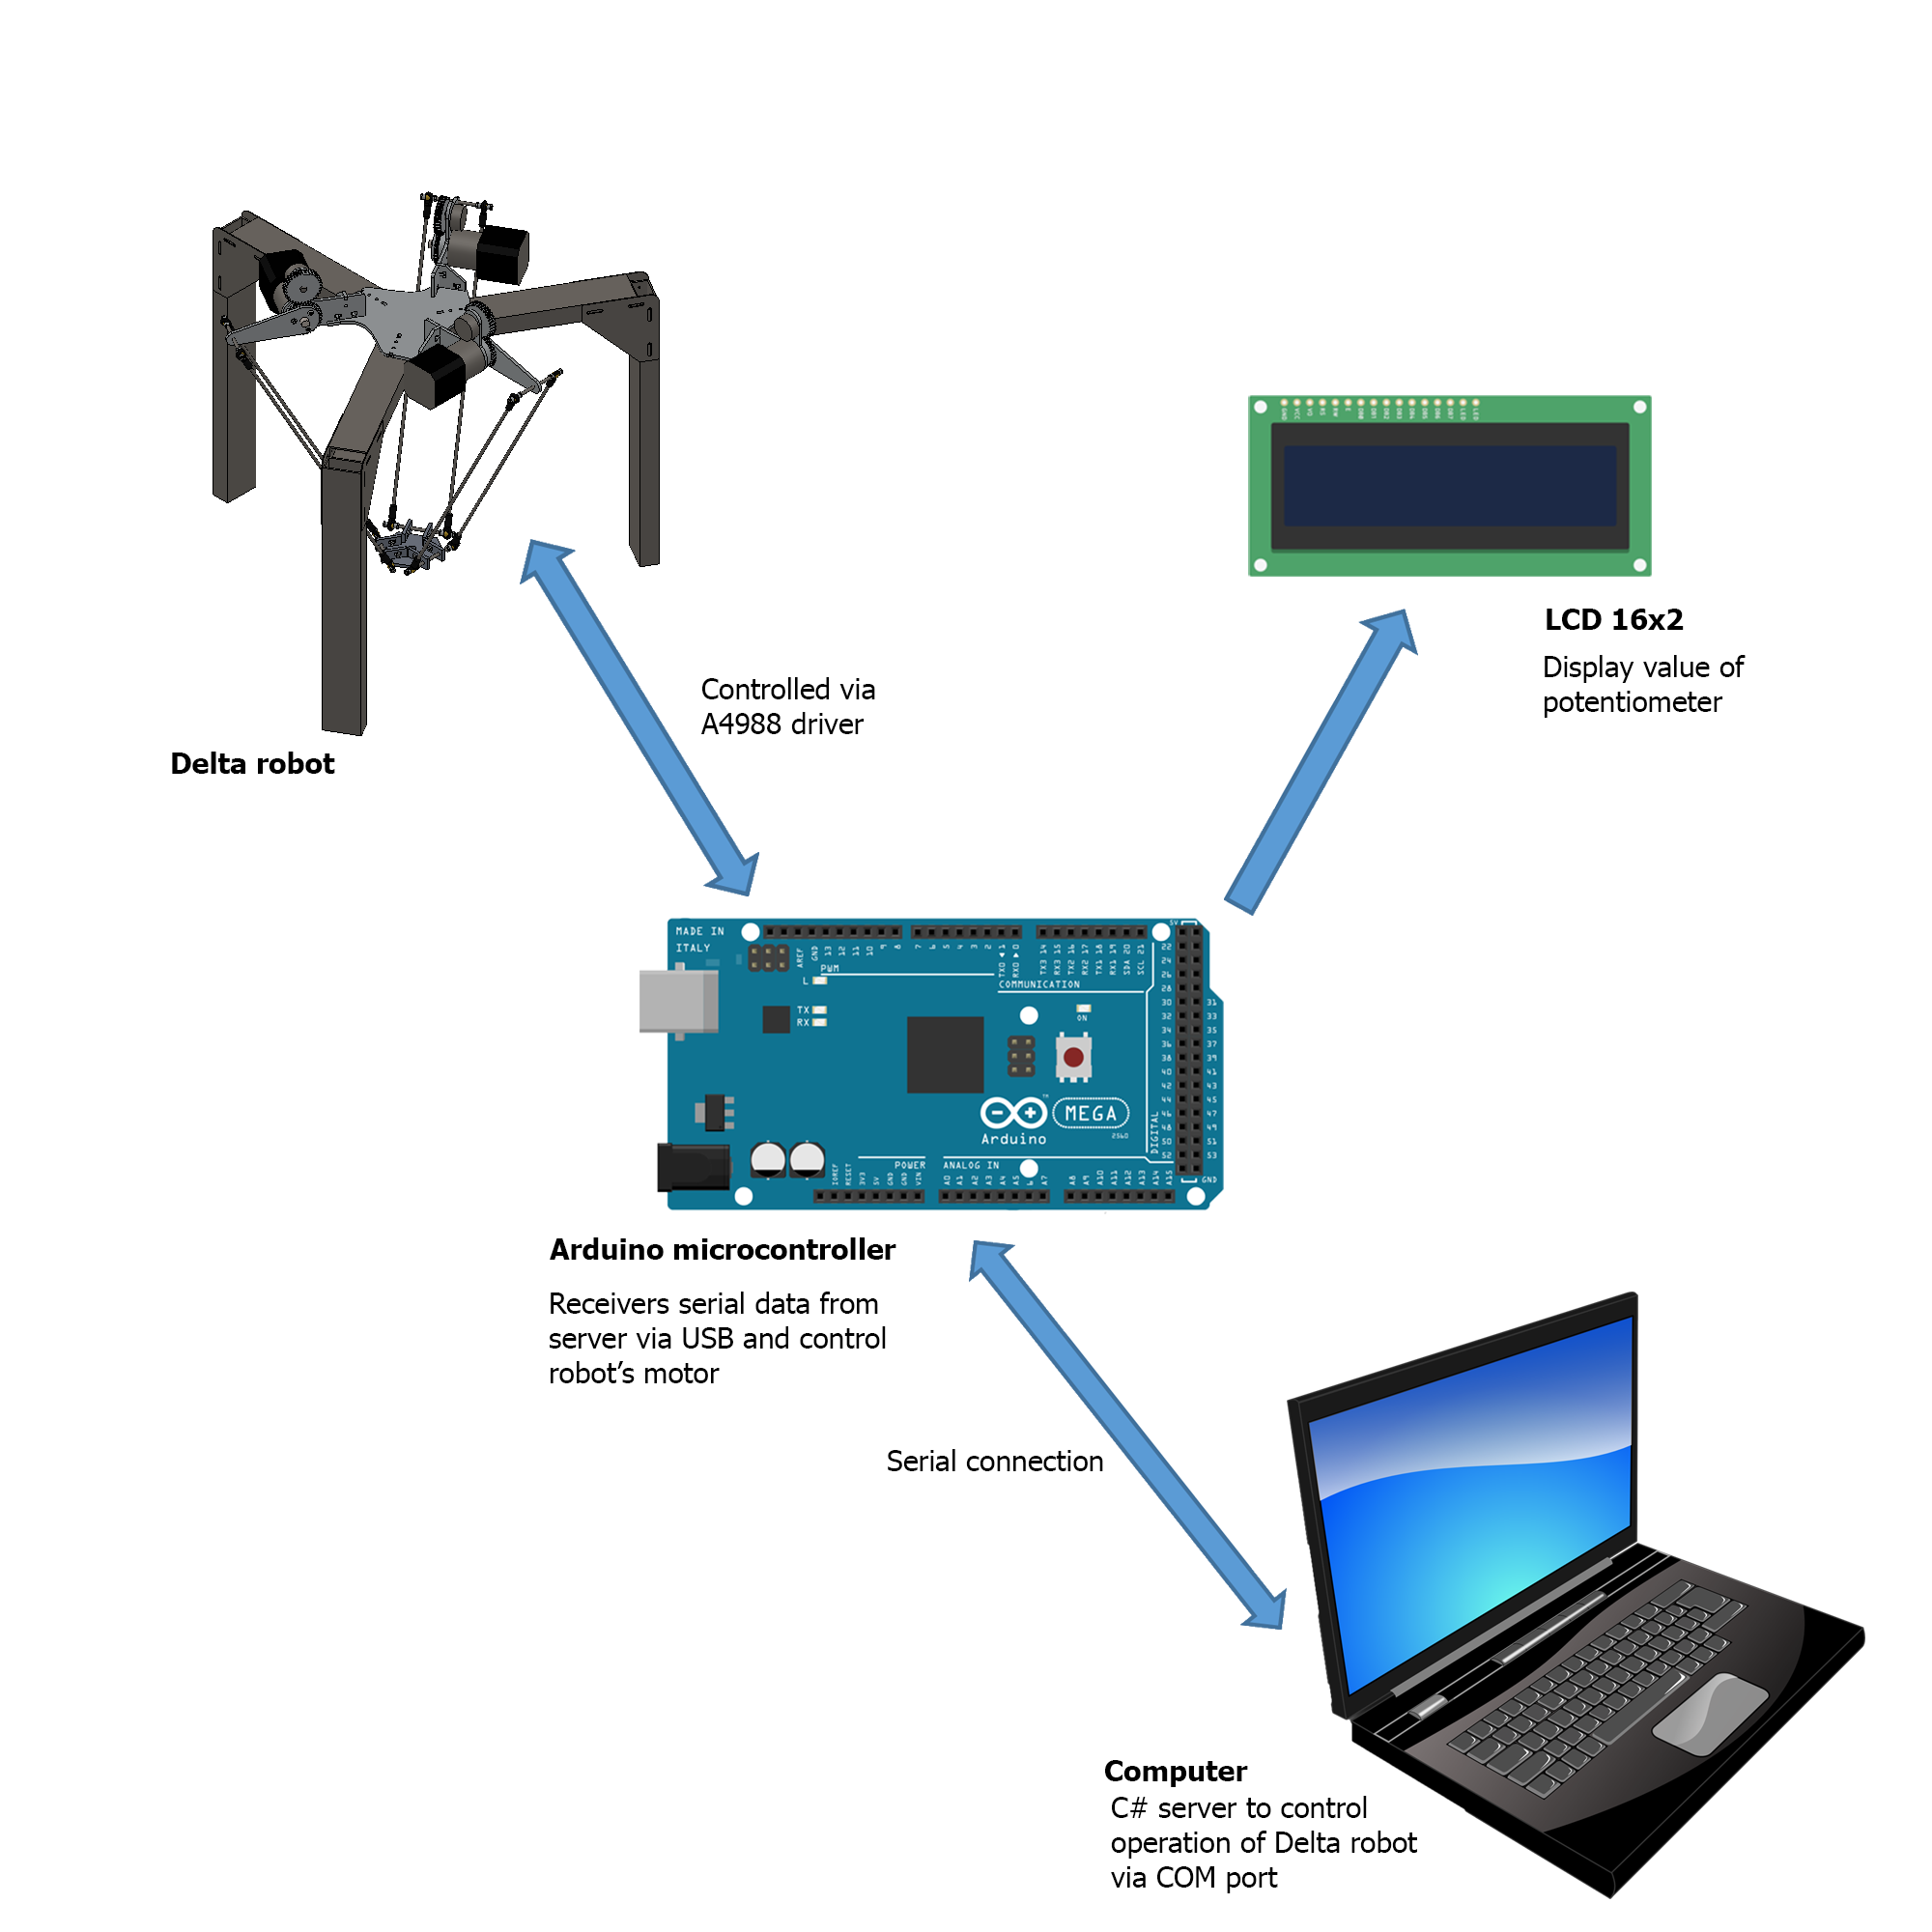
\includegraphics[width=\maxwidth{17cm}, keepaspectratio]{Chapters/Fig/system_overview.png}
	\caption{System overview}
	\label{fig:system_overview}
\end{figure}

\section{Goals of the thesis}
In order to develop a Automated Mobile App Testing System based on the Delta robot, the following objectives are proposed:
	\begin{itemize}
		\item[--] Choosing a Robotic Platform.
		\item[--] Design and manufacture hardware.
		\item[--] Creating control library(API).
	\end{itemize}

\section{Outline of thesis}

In first two chapters, I will be dealing with technologies and tools supporting Delta Robot which include theoretical background and implementation in the project.
In the third chapter, I present the design of hardware and software of the robot.

And the next chapter describes practical experiments with the system and our evaluation on the results. Thus can assess the accuracy and reliability of the system.

In general, the whole thesis aims mainly to build mini delta robot for automated mobile app testing system. \nocite{radim_thesis}